\chapter{Evaluation}

To evaluate our system we run some tests on Microworkers. In this section we introduce the settings and take a look at the results from our tests.

\section{First Tests}\label{sec:firstTest}

To get a first impression how good the answers from Microworkers are we wanted to create first a basic system to test the workers and to learn where the problems in the system are.

\subsection{Setting}
The first test evaluates the system in a basic setting. For this purpose, we used the preliminary layout as described in Section \ref{sec:FirstLayout}.
To explain the task in more detail to the users, a tutorial document (Appendix A) was created, which is linked to the campaign description on Microworkers.\newline
\newline
In this first system, users only had to select the time, the team, and the event for all events in a 5 second video snippet, where all users got a different sequence.
The events have been reduced to:
\begin{itemize}
	\setlength{\itemsep}{1pt}
	\setlength{\parskip}{1pt}
	\item Pass
	\item Foul
	\item Out
	\item Corner Kick
	\item Shot off target
	\item Shot on target
	\item Goal
	\item Card
\end{itemize}

Data was gathered from 84 users of the Microworkers platform, where each second of the video is annotated by 5 workers.


\subsection{Results}

To evaluate the results of the first test, the data entered by the workers to the video file was compared manually.
With those results we decided if a user is accepted and, thus, receives his payment.
It took about 20 hours to be finished with all 55 task.

\begin{figure}[H]
    \centering
    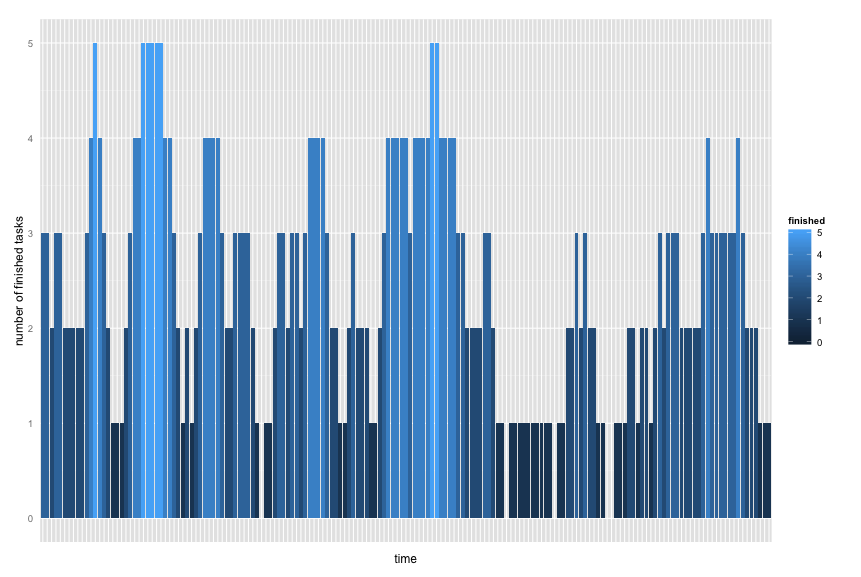
\includegraphics[width=0.9\textwidth]{firsttest/Missed_sum}
    \caption{Number of finished tasks per second of first test}
    \label{fig:MissedSum}
\end{figure}

Figure \ref{fig:MissedSum} shows there are parts of the sequence that are not annotated, because some users start a task and do not finish it. Of all 169 tasks received, only 84 were finished, which is almost $50\%$.

Of those 84 finished tasks, 53 were accepted and the other 31 tasks were not; this is about $37\%$ that were not accepted.
The tasks were not accepted for various reasons: First, some completed tasks did not contain any events but were marked by the worker as finished. Second, there were tasks that contained completely wrong data, where users missundestood the task and entered just events for almost every second. Third, many workers were just entering one or two events where should be more. Fourth, the data was in some cases very inaccurate regarding the timing of the event.

\subsection{Conclusion}

As a consequence of the first evaluation, changes were made to the system and the user interface: 

First, the layout was changed to a more guided version and a prompt was added telling workers to check the sequence for more events, because many users had not entered all events in sequence, mostly only entered the first one.

Second, the system for generating the tasks was changed so that users can be previously assigned to them, because, as can be seen in Figure \ref{fig:MissedSum}, nearly all video seconds do not consist of the required five user data entries.

Third, the explanation sheet was removed and a tutorial movie explaining the task was added instead.

\newpage
\section{Pretest}\label{sec:pretest}

For further tests, the layout was changed to the second layout approach described in Section \ref{sec:SecondLayout}. A PDF file explaining the system was discarded and the instructions were integrated into a tutorial video, which is displayed as an overlay at first when entering the web page.

\subsection{Setting}

The second test introduced a new user interface more guided than the first one, as described in Section \ref{sec:SecondLayout}.

Compared to the first test, workers now also have to enter a positional data and  some more events were added to the event list.
\newline

To explain the layout and the task they have to do, every user  will see a tutorial video at the beginning. In this video, the layout and the task of every user are explained.
\newline
To get a first rating of every user, all users have to do a pretest against a ground truth, the pretest uses the same sequence for all users.

With the test against the ground truth the rating of each event and every users first task is calculated, as described in Section \ref{RatingSystem}.

\subsection{Results}

Out of 709 users who participated in the pretest, 278 scored well enough to be allowed to enter data in the true test.


\begin{figure}[H]
    \centering
    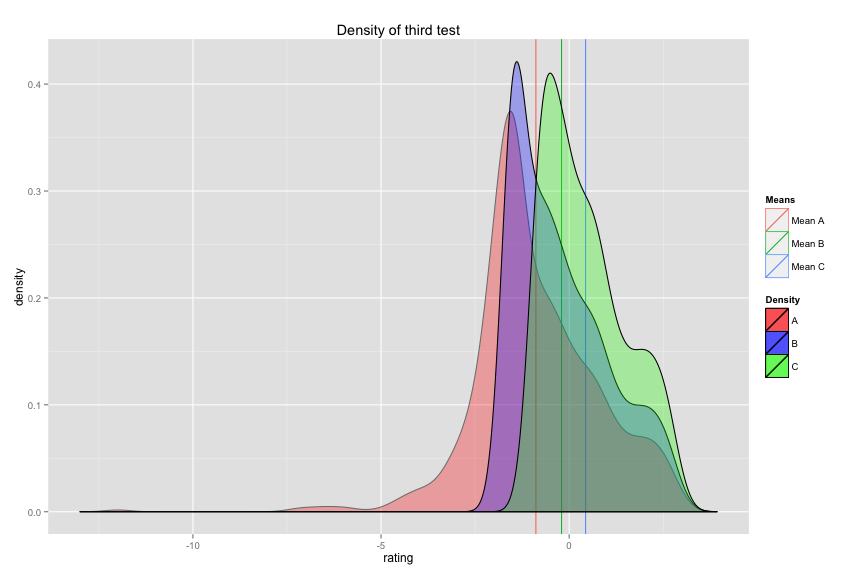
\includegraphics[width=0.9\textwidth]{pretest/Density_pretest.png}
    \caption{Densities of the pretest with a different minimum of rating (mean of A $= -0.88$, mean of B $ = -0.20$ and the mean of C is $0.44$)}
    \label{img:Density_pretest}
\end{figure}

\begin{figure}[H]
    \centering
    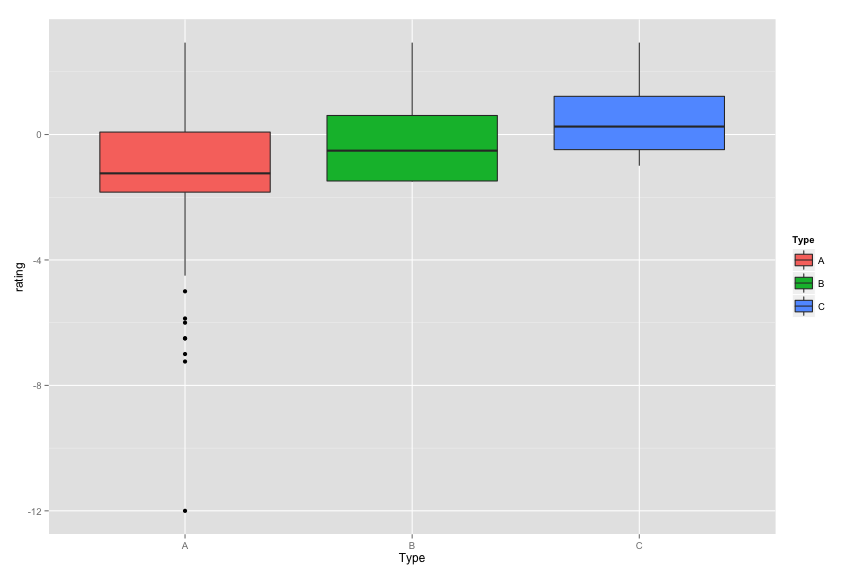
\includegraphics[width=0.9\textwidth]{pretest/Boxplot_pretest.png}
    \caption{Boxplot with task-ratings of pretest}
    \label{img:Boxplot_pretest}
\end{figure}

Figures \ref{img:Density_pretest} and \ref{img:Boxplot_pretest} show the data of all finished tasks: B shows all tasks of the pretest where the rating is larger than -1.5, which are all accepted tasks. C shows all values larger than -1; users with a pretest rating greater than -1 are accepted to do further tasks.

\begin{figure}[H]
    \centering
    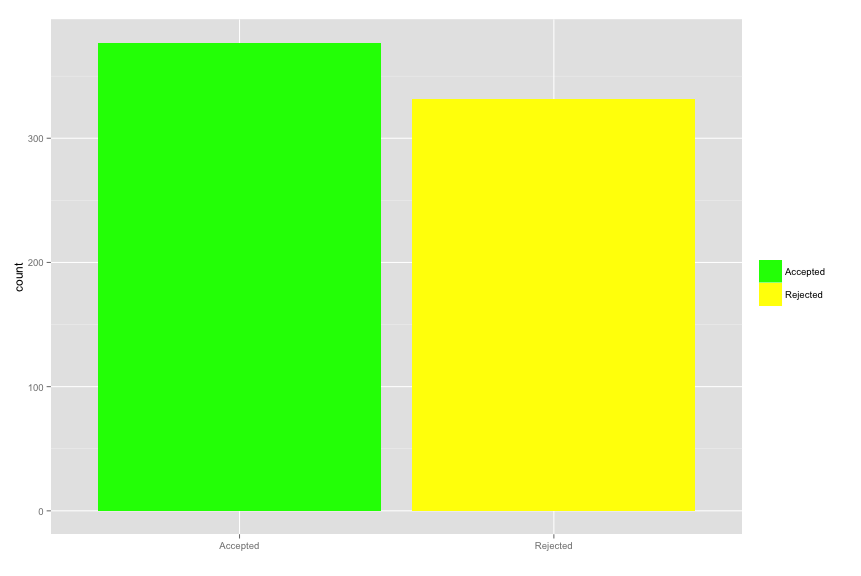
\includegraphics[width=0.9\textwidth]{pretest/Accepted_Rejected}
    \caption{Accepted and rejected number of tasks in the pretest}
    \label{img:accepted:rejected:Pretest}
\end{figure}

As shown in Figure \ref{img:accepted:rejected:Pretest}, $377$ tasks out of $709$ were accepted, which is an acceptance rate of $53\%$. The average rating of those 377 tasks was $0.22$ and the average rating of all tasks with a rating $>$ 0 was $1.17$.

\begin{figure}[H]
    \centering
    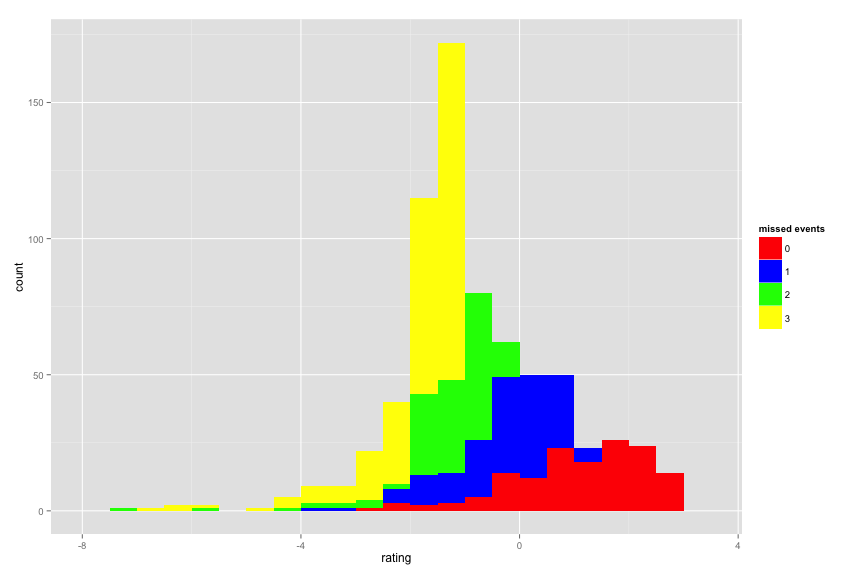
\includegraphics[width=0.9\textwidth]{pretest/Missed_pretest}
    \caption{Missed events in the pretest}
    \label{img:missedPretest}
\end{figure}

Comparing the missed events with the rating, it can be seen that even if people miss 2 events they can get a rating of 0 which is the average of all accepted event ratings and neither good nor bad.
However, even with 0 missed events out of 3, people can get a rating smaller than $-1$, those people with such a rating and 0 missed events just worked really inexactly.
If we look at the number of tasks considering the missed events with a rating $\ge 0$, there are $117$ tasks with 0 missed events and $70$ tasks with missed events $= 1$.
Considering all tasks with a rating $\ge 1$, only $5,75 \%$ have one missed event, all others are without any missed events.


\begin{figure}[H]
    \centering
    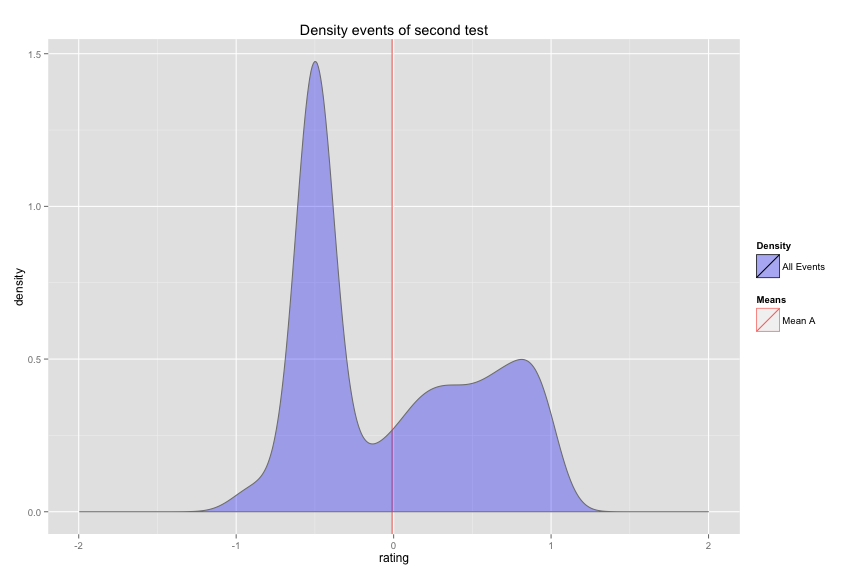
\includegraphics[width=0.9\textwidth]{pretest/DensityEvents_pretest}
    \caption{Density of all events in the pretest (mean of A $= - 0.009$)}
\end{figure}

\begin{figure}[H]
    \centering
    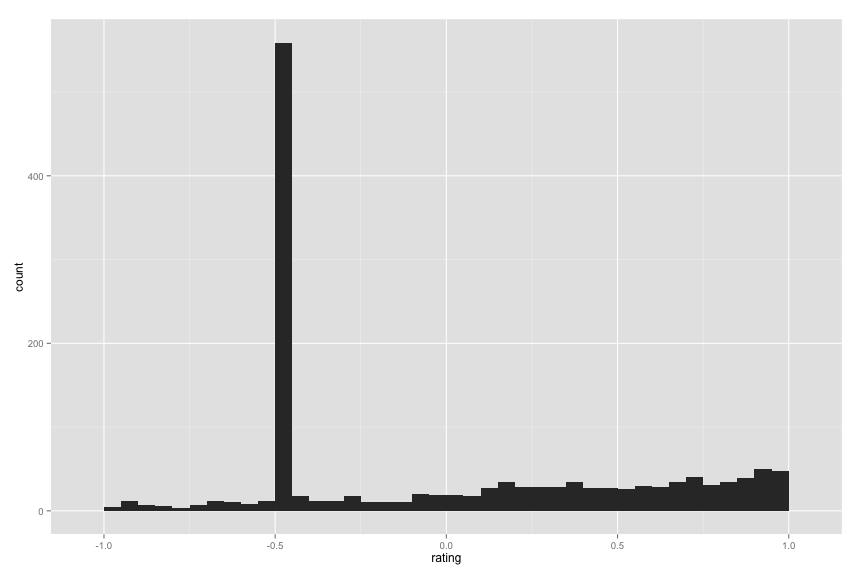
\includegraphics[width=0.9\textwidth]{pretest/HistogramEvents_pretest}
    \caption{Distribution of the rating of pretest}
\end{figure}

The total number of added events in these 709 tasks was 1406, which means that the average task contained about $1.98$ events, whereas it should contain 3 events.
Looking at the distribution of the ratings of the pretest, there are $550$ added events with a rating of $-0.5$, which means that the added event did not correspond to any event in this sequence. This means that $39.12\%$ of all added events are wrong.

\subsection{Conclusion}

This second test showed that almost half of the persons had a rating of $\le$ -1.5. This means that they are not allowed to do further tasks. Those users have not received their token after finishing their first task and therefore they were not paid.
According to the introduced rating system, users that score this badly are no longer allowed to participate in the tasks involving the true data and will, thus, not be payed for wrong work.

Figure \ref{img:Density_pretest} shows that, when excluding users with bad rating from further tasks, the average rating of users in the task increases from $-0.88$ to $0.44$, which is a difference of 1.32.

It is also discovered that there is a correlation between the number of missed events and the rating. All people who missed three events will not be able to do more tasks. In addition, 42 of 143 people with two missed events will also be disqualified from doing more tasks, because their entered values scored too low.


\newpage

\section{Evaluation of Data Integration and Cleaning}

In this part of the evaluation, the system running the DBSCAN and UPGMA algorithm is tested and the performance output is compared with manually entered data.

For more meaningful results, only sequences of the game without any replay clips or slow motion views were accepted for all the tests.


\subsection{First test}
In the first test, a sequence of 50.5 seconds was chosen, which will result in 101 tasks.
The sequence started at minute 33 and 50 seconds and ended with the beginning of the last task at 34:40.

\paragraph{Results}

\begin{figure}[H]
    \centering
    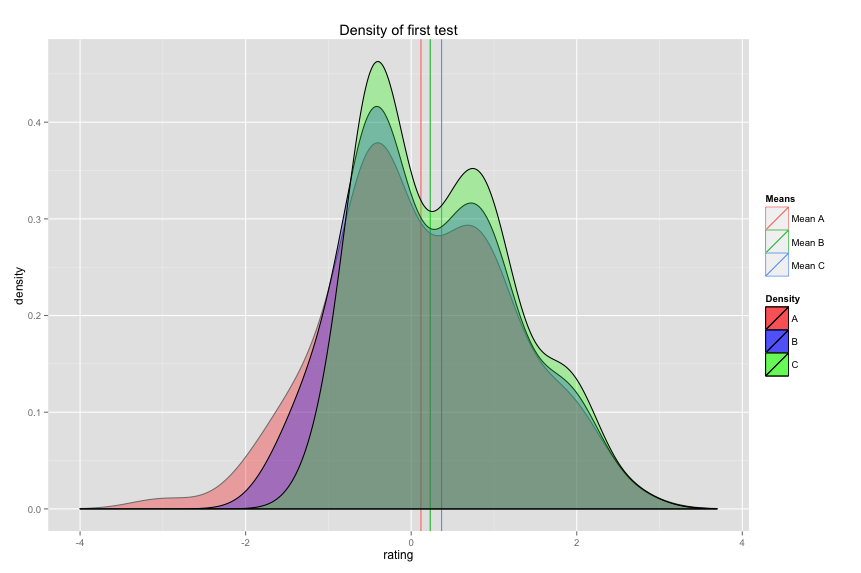
\includegraphics[width=0.9\textwidth]{standard/firsttest/Density_firsttest.png}
    \caption{Densities of the first with a different minimum of rating (mean of A is $0.12$, the mean of B is $0.23$ and the mean of C $ = 0.37$)}
\end{figure}

\begin{figure}[H]
    \centering
    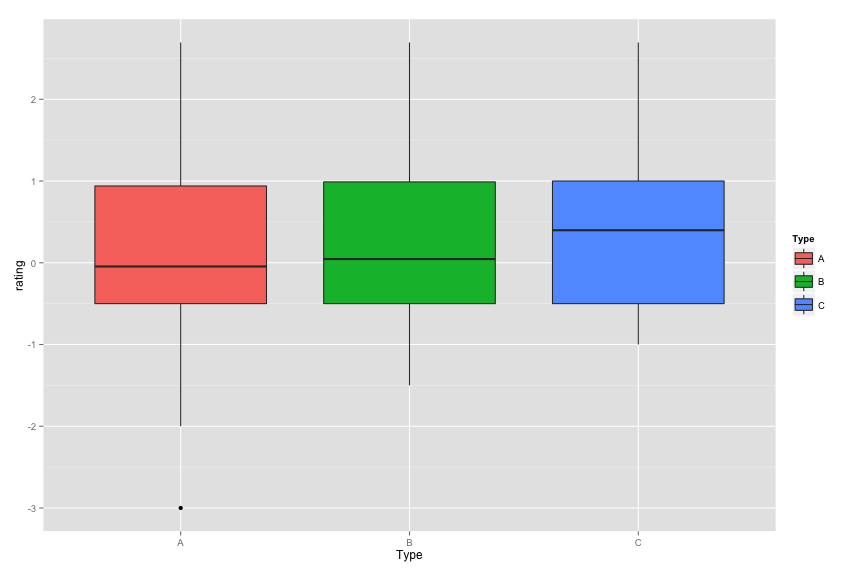
\includegraphics[width=0.9\textwidth]{standard/firsttest/Boxplot_firsttest.png}
    \caption{Boxplot with task-ratings of first test}
\end{figure}

As shown in the figures below, all means in this second campaign $\ge 0$.\newline

\begin{figure}[H]
    \centering
    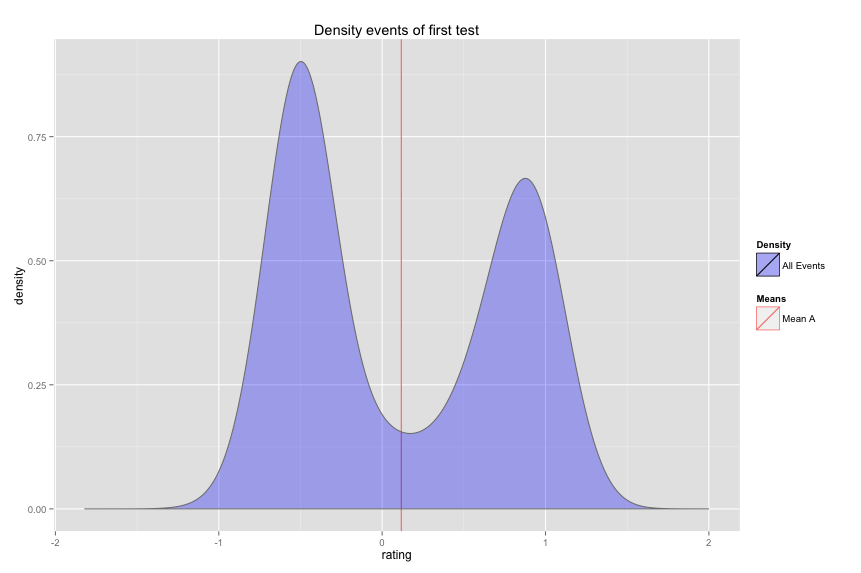
\includegraphics[width=\textwidth]{standard/firsttest/DensityEvents_firsttest.png}
    \caption{Density of all events in the first test (mean of A is $0.12$)}
    \label{img:DensEvents:first}
\end{figure}

\begin{figure}[H]
    \centering
    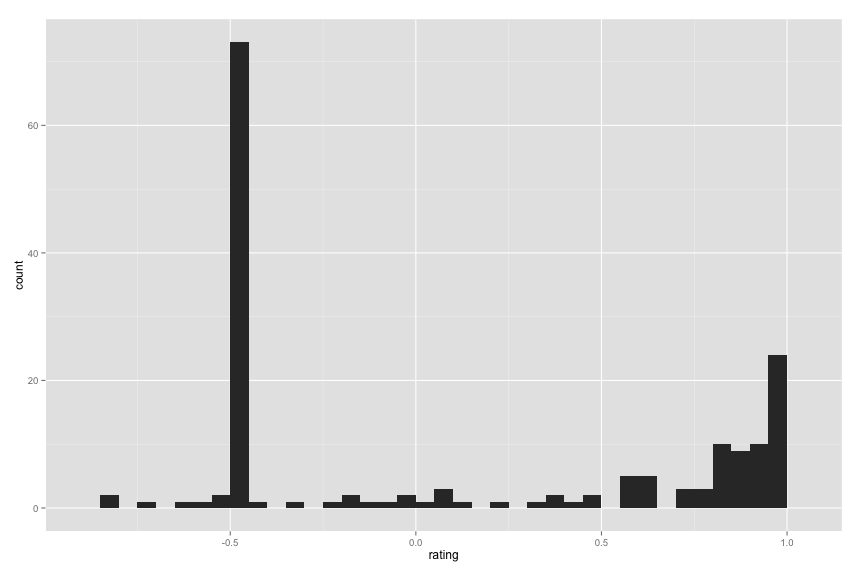
\includegraphics[width=\textwidth]{standard/firsttest/HistogramEvents_firsttest.png}
    \caption{Histogram, distribution of event-ratings}
    \label{img:HistEvent:first}
\end{figure}

In Figures \ref{img:DensEvents:first} and \ref{img:HistEvent:first}, the total number of added events in this second campaign is 170, which results in an average of $1.7$ events per task. We have 73 events with a rating of -0.5. This are $42.9\%$ events, which cannot be assigned to any calculated events by DBSCAN.

Looking at the difference between the points calculated with DBSCAN and the entered points, the following results were obtained.

\begin{table}[H]
    \begin{center}
		\begin{tabular}{|l|l|l|l|l}
			\hline
            \multicolumn{4}{|c|}{\large \textbf{Difference}} \\
			\hhline{====}
			\textbf{position} & \textbf{time} & \textbf{event} & \textbf{team} \\
			\hline
			12,74153052 & 0,1 & 0 & 0\\
			\hline
			34,15673433 & 0,1 & 0 & 0\\
			\hline
			17,17876014 & 0,1 & 0 & 0\\
			\hline
			5,580197129 & 0,1 & 0 & 0\\
			\hline
			15,30154567 & 0,3 & 0 & 0\\
			\hline
			7,011305157 & 0,2 & 0 & 0\\
			\hline
			\textcolor{red}{61,33984023} & 0,1 & 0 & 0\\
			\hline
			15,49588978 & 0,1 & 0 & 0\\
			\hline
			\textcolor{red}{42,52275273} & 0,2 & 0 & 0\\
			\hline
			29,19160496 & 0,1 & 0 & 0\\
			\hline
			19,57876911 & 0,2 & 0 & 0\\
			\hline
			\textcolor{red}{44,82389095} & 0,1 & 0 & 0\\
			\hline
		\end{tabular}
    \end{center}
    \caption{Difference between the calculated events and the ground truth with DBSCAN}
\end{table}

The average variance in the time is $0.15$; in the position, the average distance is $25.4$; and there are no faults in the event and the team's ID.
Looking at the red-colored positions, some values had a distance of $\ge 40$; these values are not really good, especially the value in the seventh row has a huge difference of $61.34$ units, which is $7.6\%$ of the whole field's distance.
However, there have been some missing events. The DBSCAN algorithm missed calculating 6 points and instead calculated one wrong point.

For comparing the UPGMA method to the DBSCAN method, the calculated base of UPGMA is given in the table below.

\begin{table}[H]
    \begin{center}
		\begin{tabular}{|l|l|l|l|l}
			\hline
            \multicolumn{4}{|c|}{\large \textbf{Difference}} \\
			\hhline{====}
			\textbf{position} & \textbf{time} & \textbf{event} & \textbf{team} \\
			\hline
			12,45540044 & 0,1 & 0 & 0 \\
			\hline
            32,64439462 & 0,1 & 0 & 0 \\
			\hline
            \textcolor{red}{61,27385168} & 0,5 & 0 & 0 \\
			\hline
            39,77870033 & \textcolor{red}{1,3} & 0 & 0 \\
			\hline
            29,58215847 & 0,4 & 0 & 0 \\
			\hline
            14,34155152 & 0 & 0 & 0 \\
			\hline
            36,55601866 & 0,2 & 0 & 0 \\
			\hline
			2,956010825 & 0 & 0 & 0 \\
			\hline
			\textcolor{red}{44,90069599} & 0,4 & 0 & 0 \\
			\hline
            17,27061088 & 0,5 & 0 & 0 \\
			\hline
		\end{tabular}
    \end{center}
    \caption{Difference between the calculated events and the ground truth with UPGMA}
    \label{fig:diff:first:UPGMA}
\end{table}

Table \ref{fig:diff:first:UPGMA} shows the distance between the points calculated with UPGMA and the manual data. Calculating the events, UPGMA calculated 10 data points calculated, whereas DBSCAN calculated 12. In addition, 3 wrong events have been calculated. The average positional distance of UPGMA is $36.60$ and the average difference in time is $0.74$ seconds.


\begin{figure}[H]
    \centering
    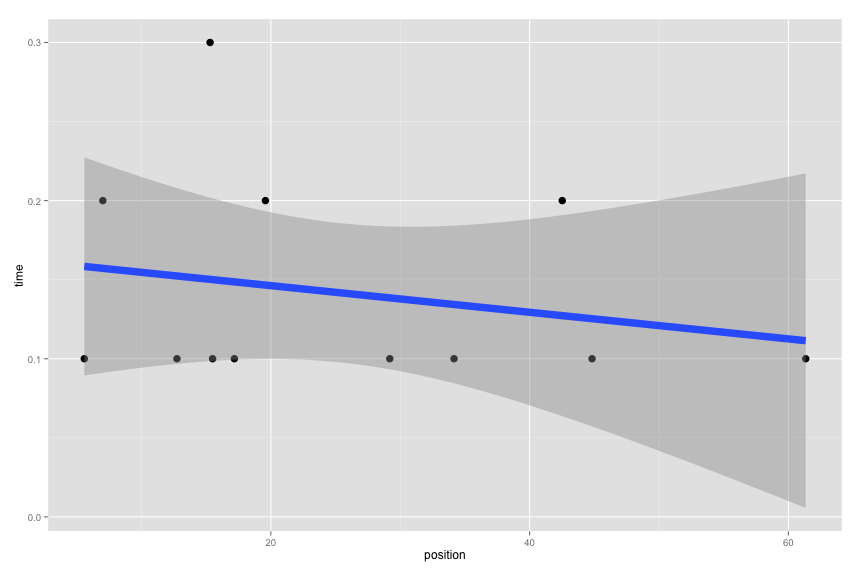
\includegraphics[width=0.9\textwidth]{standard/firsttest/Difference_firsttest}
    \caption{Correlation of the position and the time error with DBSCAN}
    \label{fig:dist_pos:first}
\end{figure}

Figure \ref{fig:dist_pos:first} shows the distance in the time and the position for each point of the calculated and allocated data-point calculated with DBSCAN. If we look at the blue line we can see that the deviation of the time do not correlate to the deviation of the position. 
\paragraph{Conclusion}
A comparison of the means with the means of the pretest shows an increase of the mean of all ratings by $1.06$ and of the mean of B by $0.5$.
This is especially significant, because both values, the mean of A and the mean of B could be raised from a negative value to a positive one.
With the mean of C, all ratings $\ge -1$ increased just by $0.2$. However, this is because in the pretest every task had three events that ended up in a maximum rating of $3.0$. Whereas, in this task every user got another task and if someone received a sequence without any events, the possible maximum rating is $1.0$, also for tasks with one event; tasks with two events leads to a maximum value of $2.0$. So the average value is smaller, because there have been 15 events in the sequence of 100 tasks where every task contains a tenth of the whole sequence, so the average event per task is only $1.5$, which is also the average maximum rating over all tasks, hereunder we got a big increase of the rating of the users, because the mean of all ratings of section A,B and C increased where at the same time the average maximum rating was half of the maximum rating in the pretest.
\newline
A comparison of the two clustering methods against each other shows that DBSCAN produces a better output regarding the number of not calculated events, the number of miscalculated events, and the difference between the calculated events.

If we take a look at the distances between the calculated and our manually entered points we can see that we did not get such a big average distance error; it is only $3.18\%$ of the whole field by calculating the base events by DBSCAN.
However, there some missed events, and those events do have different reasons why they are missing.
One point is missing because in the first and last seconds of the analyzed sequence less than 10 task are created. The DBSCAN algorithm accepts clusters with more than four points.
Another problem in the sequence is that some points exists that are too close to each other. In this sequence, there are three interceptions, where the ball gets to another player of the intercepting team. Those points have only a difference in the event types ID and will summarize to one single point with DBSCAN.

\subsection{Second test}

The evaluate the stability of the first standard test, a second campaign was created, which contained 150 tasks and was 75 seconds long.
The sequence started at minute 6 and 43 seconds and also and did not contain any repetitions or slow motion clips.

\paragraph{Results}

\begin{figure}[H]
    \centering
    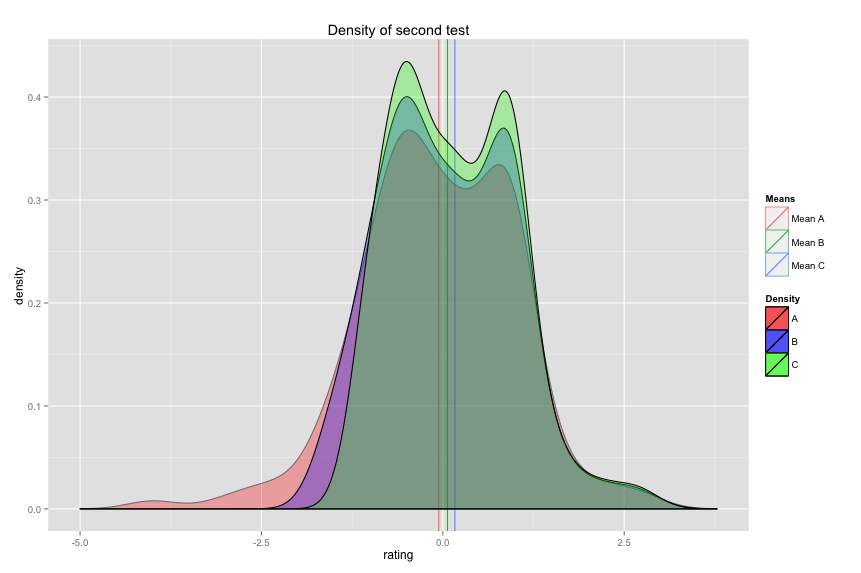
\includegraphics[width=0.9\textwidth]{standard/secondtest/Density_secondtest.png}
    \caption{Densities of the second with a different minimum of rating (mean of A is $-0.06$, the mean of B is $0.06$ and the mean of C $ = 0.17$)}
    \label{img:Density:secontest}
\end{figure}

\begin{figure}[H]
    \centering
    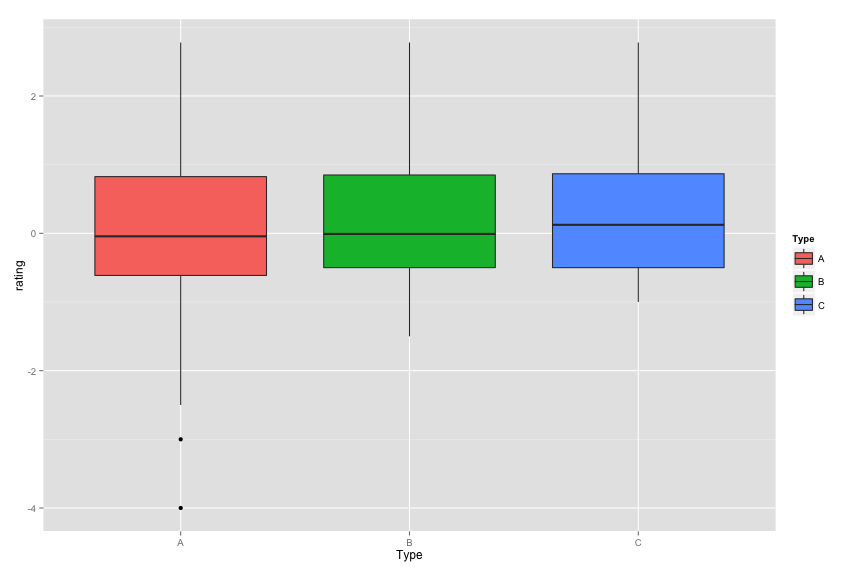
\includegraphics[width=0.9\textwidth]{standard/secondtest/Boxplot_secondtest.png}
    \caption{Boxplot with task-ratings of second test}
    \label{img:Boxplot_secondtest}
\end{figure}

As shown in Figure \ref{img:Density:secontest} after the average rating of all tasks is again negative. In addition, the boxplot in Figure \ref{img:Boxplot_secondtest} does not show a big difference between the three classes A, B and C. This is because only 13 of 150 tasks have a rating less than $-1.5$ $(8\%)$ and not many tasks have a great rating: there are only $23$ tasks with a rating $\ge 1 15$ $(3\%)$ and only $3$ tasks with a rating $\ge 2$ $(2\%)$.

\begin{figure}[H]
    \centering
    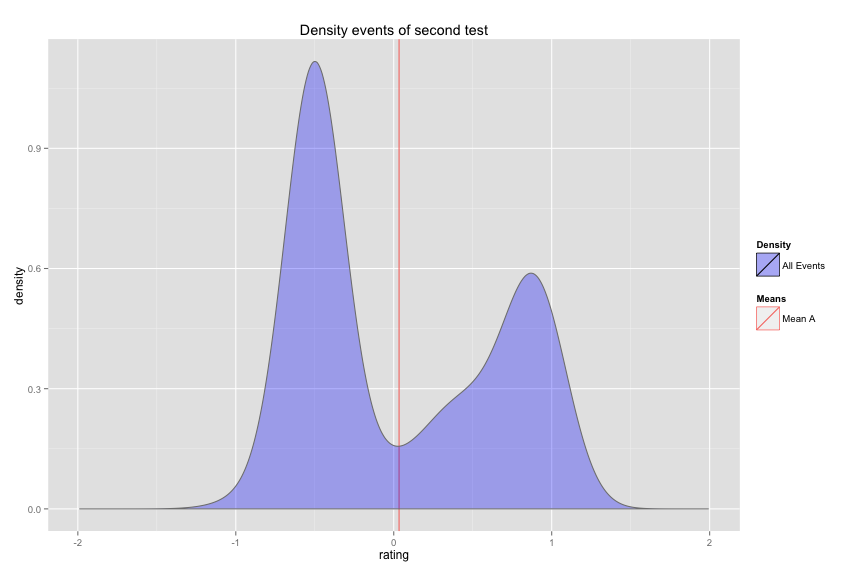
\includegraphics[width=0.9\textwidth]{standard/secondtest/DensityEvents_secondtest.png}
    \caption{Density of all events in the second test (mean of A is $0.034$)}
\end{figure}

\begin{figure}[H]
    \centering
    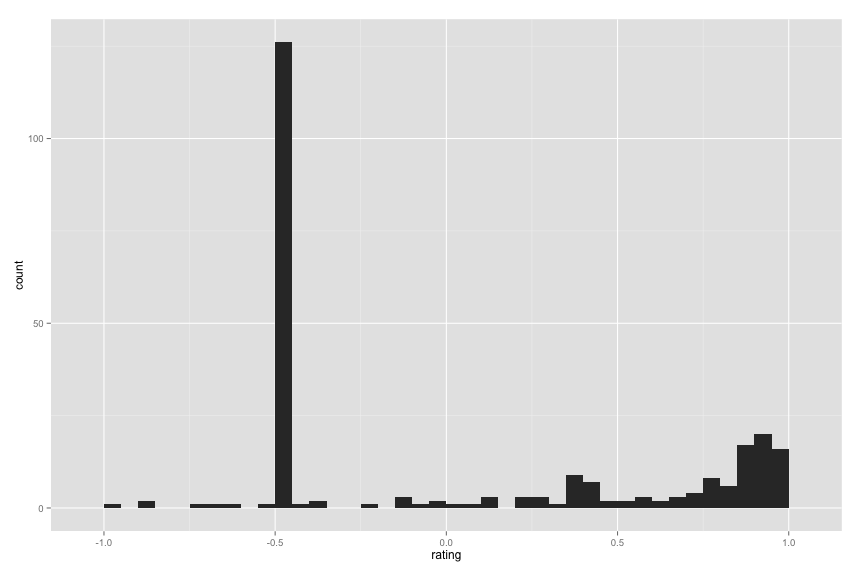
\includegraphics[width=0.9\textwidth]{standard/secondtest/HistogramEvents_secondtest.png}
    \caption{Histogram, distribution of event-ratings}
\end{figure}

$49.21\%$ cannot be assigned to any event calculated by DBSCAN. In addition, only 111 events have a rating $\ge 0$ and there are $43\%$ events with positive rating. Only $7\%$ are classified as inexact events.
\newline

\begin{table}[H]
    \begin{center}
		\begin{tabular}{|l|l|l|l|l}
			\hline
            \multicolumn{4}{|c|}{\large \textbf{Difference}} \\
			\hhline{====}
			\textbf{position} & \textbf{time} & \textbf{event} & \textbf{team} \\
			\hline
			25,34028327 & 0,17 & 0 & 0\\
			\hline
            34,30953076 & 0,05 & 0 & 0\\
			\hline
            19,63206054 & 0,13 & 1 & 1\\
			\hline
            12,67110102 & 0,91 & 0 & 0\\
			\hline
            \textcolor{red}{45,67720521} & 0 & 0 & 0\\
			\hline
            \textcolor{red}{56,70615378} & 0,27 & 1 & 1\\
			\hline
            26,34557062 & 0,92 & 1 & 0\\
			\hline
            26,65355513 & 0,12 & 0 & 0\\
			\hline
            15,68471868 & 0,08 & 1 & 1\\
			\hline
            18,0454648 & 0,1 & 0 & 0\\
			\hline
            17,06519557 & 0,18 & 0 & 0\\
			\hline
            \textcolor{red}{46,75355922} & 0,08 & 1 & 1\\
			\hline
            15,40143175 & 0,21 & 0 & 0\\
			\hline
            6,860466456 & 0,08 & 0 & 0\\
			\hline
            17,72570419 & 0,6 & 1 & 0\\
			\hline
		\end{tabular}
    \end{center}
    \caption{Difference between the calculated events and the ground truth with UPGMA}
    \label{fig:diff:sec:UPGMA}
\end{table}

Table \ref{fig:diff:sec:UPGMA} shows the difference between the UPGMA calculated events and the manual events. Only 3 events have a big positional distance. The worst thing of this test is that 19 events were not calculated and only 15 were calculated.


\begin{table}[H]
    \begin{center}
		\begin{tabular}{|l|l|l|l|l}
			\hline
            \multicolumn{4}{|c|}{\large \textbf{Difference}} \\
			\hhline{====}
			\textbf{position} & \textbf{time} & \textbf{event} & \textbf{team} \\
			\hline
			25,34028327 & 0,17 & 0 & 0\\
			\hline
            \textcolor{red}{40,68001028} & 0,13 & 1 & 0\\
			\hline
            27,97846143 & 0,16 & 0 & 0\\
			\hline
            39,41173937 & 0,19 & 0 & 0\\
			\hline
            17,31048899 & 0,02 & 0 & 0\\
			\hline
            9,638692287 & 0,12 & 0 & 0\\
			\hline
            22,65005439 & 0,72 & 1 & 0\\
			\hline
            \textcolor{red}{47,12557526} & 0,39 & 0 & 0\\
			\hline
            18,08048698 & 0,47 & 1 & 0\\
			\hline
            23,87727198 & 0,33 & 0 & 0\\
			\hline
            18,86387553 & 0,18 & 1 & 1\\
			\hline
            28,64668393 & 0,26 & 0 & 0\\
			\hline
            13,13141653 & 0,19 & 1 & 0\\
			\hline
            \textcolor{red}{59,98198396} & 0,03 & 0 & 0\\
			\hline
            17,61656323 & 0,4 & 0 & 0\\
			\hline
            11,83990287 & 0,15 & 0 & 0\\
			\hline
            25,14386207 & 0,4 & 1 & 0\\
			\hline
		\end{tabular}
    \end{center}
    \caption{Difference between the calculated events and the ground truth with DBSCAN}
\end{table}

The comparison of the calculated events of this sequence to the manually added values shows an average position error of $26.31$. However, four values are larger than 40 units, with an average distance of $49.26$. The average time deviation in the second campaign is $0.254$, which is neither bad nor good.
A big difference compared to the first task is that that here six wrong events and one wrong team were calculated. Six wrong events are $35.29\%$ wrong events.
Another problem in this second campaign is that DBSCAN calculated 17 events, whereas  34 events were added manually, which means that $50\%$ of all tasks were missed.

Sorting the data by the rating, where the biggest rating comes first, results in some other, better values:

\begin{table}[H]
    \begin{center}
		\begin{tabular}{|l|l|l|l|l}
			\hline
            \multicolumn{4}{|c|}{\large \textbf{Difference}} \\
			\hhline{====}
			\textbf{position} & \textbf{time} & \textbf{event} & \textbf{team} \\
			\hline
            26,00076922	& 0,17 & 0 & 0\\
			\hline
            26,41113167 & 0,39 & 0 & 0\\
   			\hline
            20,21594482 & 0,19 & 0 & 0\\
			\hline
            27,31117949 & 0,25 & 0 & 0\\
			\hline
            5,28924229 & 0,06 & 0 & 0\\
			\hline
            18,00972584 & 0,27 & 1 & 1\\
			\hline
            12,99650572 & 0,39 & 0 & 0\\
			\hline
            39,56039054 & 0,63 & 0 & 0\\
			\hline
            17,22161575 & 0,32 & 0 & 0\\
			\hline
            53,87906387 & 0,37 & 0 & 1\\
    			\hline
            16,0350469 & 0,06 & 0 & 0\\
			\hline
            28,03882688 & 0,13 & 0 & 0\\
			\hline
            15,43160717 & 0,09 & 1 & 0\\
			\hline
            19,41012622 & 0,11 & 0 & 0\\
			\hline
            \textcolor{red}{41,79745686} & 0,3 & 0 & 0\\
			\hline
            30,81527057 & 0,43 & 0 & 0\\
			\hline
            15,68963033 & 0 & 0 & 0\\
			\hline
            6,579004484 & 0,07 & 0 & 0\\
			\hline
            30,52929413 & 0,35 & 1 & 0\\
			\hline
		\end{tabular}
    \end{center}
    \caption{Difference between the calculated events and the ground truth, with respect to the rating}
    \label{img:diffGT:second:ordered}
\end{table}


By sorting those values, the number of events can be decreased, with a difference in the position $\ge 40$, as visible in Figure \ref{img:diffGT:second:ordered}. 
The number of not calculated tasks can also be reduced from 17 to 14 and the average position error can be decreased to $23.74$ units.
The number of wrong teams could be decreased from six to three and the number of wrong teams increased from one to two, by the DBSCAN calculations.
Now, just one calculated point exists that does not belong to a manually entered data, whereas, in the by time ordered case it has been two.


\begin{figure}[H]
    \centering
    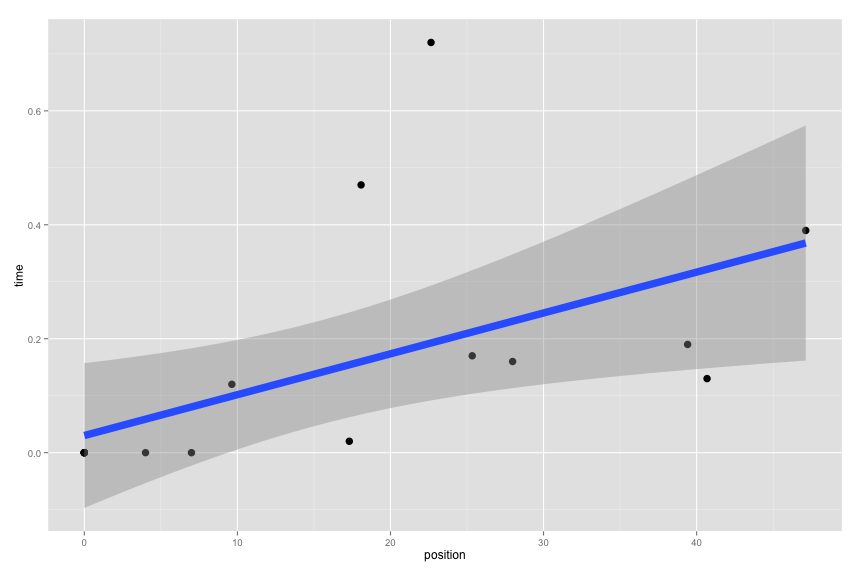
\includegraphics[width=\textwidth]{standard/secondtest/Difference_secondtest.png}
    \caption{Correlation of position and time}
    \label{img:correlation:second}
\end{figure}

\begin{figure}[H]
    \centering
    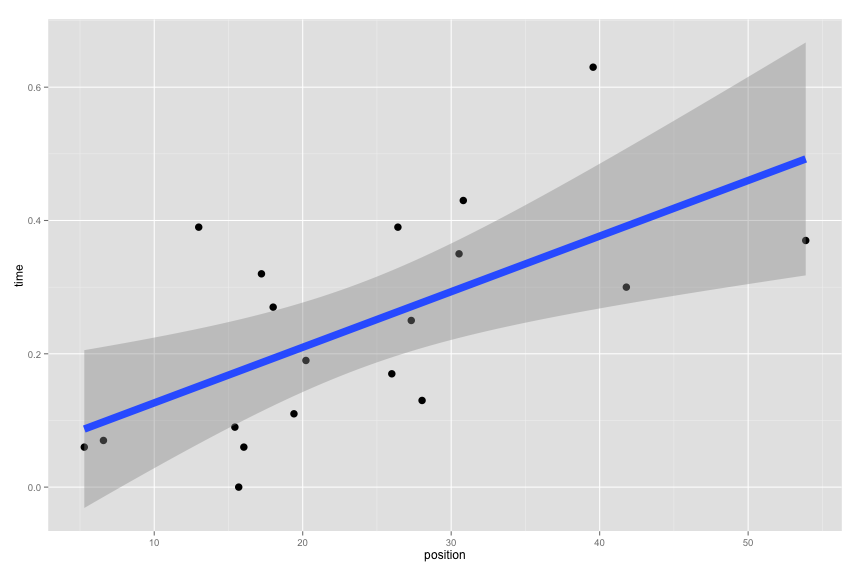
\includegraphics[width=\textwidth]{standard/secondtest/DifferenceOrdered_secondtest.png}
    \caption{Correlation of position and time with ordered method}
    \label{img:correlation:ordered:second}
\end{figure}

As shown in Figures \ref{img:correlation:ordered:second} and \ref{img:correlation:second}, there is a correlation between the distance of the position and the distance in the time in both DBSCAN methods. In addition, near position values in this test have close time values, and big position error values have bigger time errors.

\paragraph{Conclusion}
In a sequence of close events, the DBSCAN algorithm cannot calculate all events. Changing the parameters was attempted, but having fewer not calculated events will increase the number of wrongly calculated events.
In the end, it is better to calculate fewer wrong events, will be interpolated in the SportSense application \cite{AlKabary:2013}.

Because sorting the values by rating got better results, it is first checked if there are enough points similar to the point with the biggest user rating. With this change, the users can be rated with good entered results.
We also compared the calculated events with the UPGMA algorithm. However, calculating the points with the UPGMA will only produce 14 points, which is less than half of all points that should be in this sequence.



\subsection{Third test}
Two take another look at our system we created another campaign of 160 tasks and 80 seconds evaluated of the soccer game.



\paragraph{Results}

\begin{figure}[H]
    \centering
    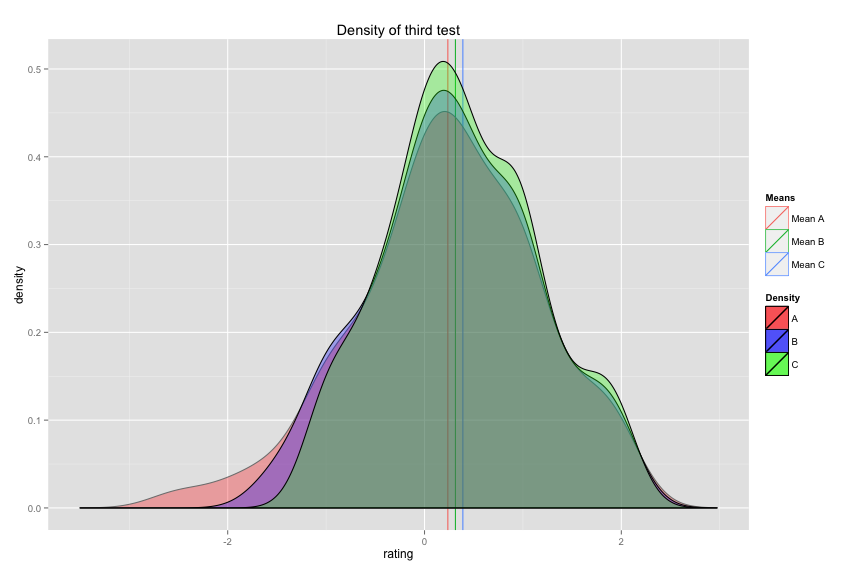
\includegraphics[width=0.9\textwidth]{standard/thirdtest/Density_thirdtest.png}
    \caption{Densities of the third with a different minimum of rating (mean of A is $0.24$, the mean of B is $0.31$ and the mean of C $ = 0.39$)}
    \label{img:Density:thirdtest}
\end{figure}

\begin{figure}[H]
    \centering
    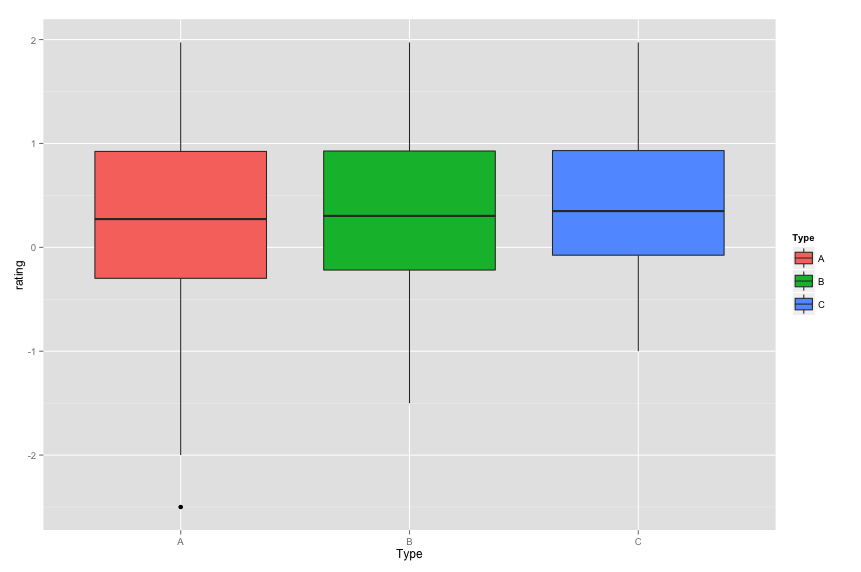
\includegraphics[width=0.9\textwidth]{standard/thirdtest/Boxplot_thirdtest.png}
    \caption{Boxplot with task-ratings of third test}
    \label{img:Boxplot_thirdtest}
\end{figure}

In Figures \ref{img:Boxplot_thirdtest} and \ref{img:Density:thirdtest} show that the upper quartile of all three sections is almost the same. The number of bad tasks is also not big.
Of the 160 tasks in this campaign, $98$ have a rating bigger than zero, which are $61,3\%$, and only $7.5\%$ of the tasks are rated less than zero.

\begin{figure}[H]
    \centering
    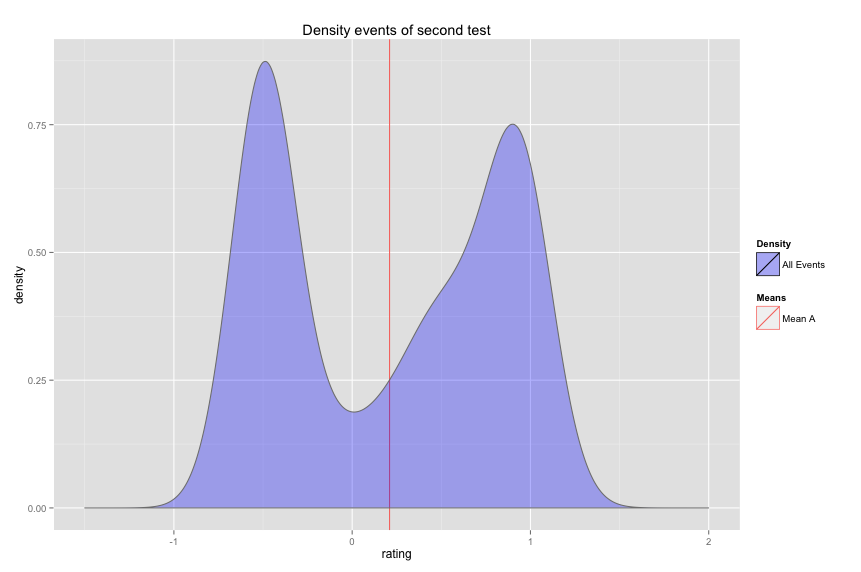
\includegraphics[width=0.9\textwidth]{standard/thirdtest/DensityEvents_thirdtest.png}
    \caption{Density of all events in the third test (mean of A is $0.034$)}
\end{figure}

\begin{figure}[H]
    \centering
    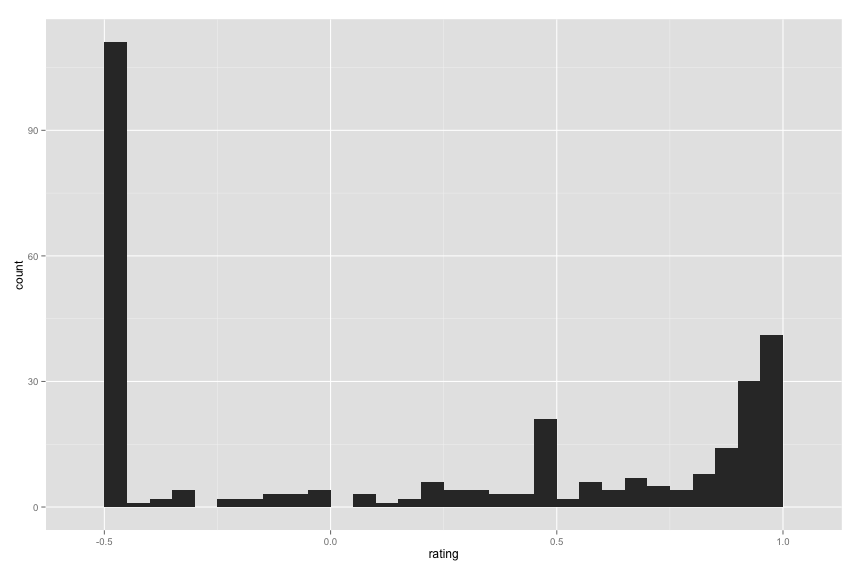
\includegraphics[width=0.9\textwidth]{standard/thirdtest/HistogramEvents_thirdtest.png}
    \caption{Histogram, distribution of event-ratings}
\end{figure}

In this campaign, the worst task rating is $-0.5$, which means that there are no inexact tasks in the users' events entered, either they are good or not classified.
Of the 300 entered events in this campaign, which makes an average of 1.9 entered events per task, 110 events have been rated by $-0.5$. These are $35\%$ of entered events, which are not assigned to a calculated event.

\begin{table}[H]
    \begin{center}
		\begin{tabular}{|l|l|l|l|l}
			\hline
            \multicolumn{4}{|c|}{\large \textbf{Difference}} \\
			\hhline{====}
			\textbf{position} & \textbf{time} & \textbf{event} & \textbf{team} \\
			\hline
			31,53933446 & 0,024 & 1 & 1 \\
			\hline
            11,95378601 & 0,143 & 0 & 0 \\
			\hline
            29,64488234 & 0,022 & 0 & 0 \\
			\hline
            10,41910793 & 0,033 & 0 & 0 \\
			\hline
            \textcolor{red}{94,67647828} & 0,005 & 0 & 0 \\
			\hline
            10,36997589 & 0,124 & 0 & 0 \\
			\hline
            21,30458085 & 0,099 & 0 & 0 \\
    			\hline
            \textcolor{red}{47,48483439} & 0,944 & 0 & 0 \\
			\hline
            33,65193326 & 0,052 & 0 & 0 \\
			\hline
            29,08902652 & 0,205 & 0 & 0 \\
			\hline
            \textcolor{red}{47,58417537} & 0,409 & 1 & 0 \\
			\hline
            9,758888922 & 0,094 & 0 & 0 \\
			\hline
            \textcolor{red}{48,20682103} & 0,899 & 0 & 0 \\
			\hline
            \textcolor{red}{44,5881021} & 0,022 & 0 & 0 \\
			\hline
            12,85083055 & 0,231 & 0 & 0 \\
			\hline
		\end{tabular}
    \end{center}
    \caption{Difference between the calculated events and the ground truth}
    \label{img:diffGT:third}
\end{table}

Figure \ref{img:diffGT:third} shows the differences between the calculated events by DBSCAN and the manually entered data.
The average distance of all entered events in this test is $32.21$ which is not really  good. However, the temporal distance does not indicate a big difference between the two related events; the average is only 0.22 seconds.
In addition, there are only four missing events, where two of them are in the first two seconds and refer to the calculation problem of DBSCAN that there must be a minimum number of points.
There is no event calculated that does not exist in the sequence.


\newpage
\section{Demographics}\label{sec:analytics}

Google Analytics\footnote{http://www.google.com/intl/de/analytics/} is a framework created by Google that generates the traffic and the traffic's source on a specified website. This tool will be used in the present approach to get an insight of users' home countries and to get an impression how long users stay on SportSense Crowdapp.

\subsection{Geographic distribution}

\begin{figure}[H]
    \centering
    \includegraphics[width=\textwidth]{geo/geoDistribution}
    \caption{Home countries of participators on SportSense Cloudapp}
    \label{fig:geoDist}
\end{figure}

\begin{figure}[H]
    \centering
    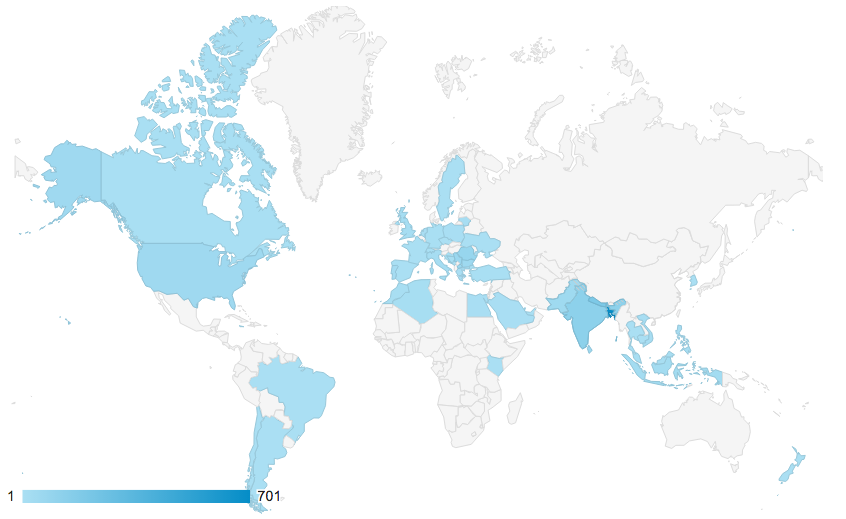
\includegraphics[width=0.9\textwidth]{geo/Landmark.png}
    \caption{Map showing the distribution of our workers}
    \label{fig:map}
\end{figure}

As can be seen in Figure \ref{fig:geoDist} and \ref{fig:map}, a majority (1697) of participants in the campaigns are from Bangladesh. This is about $41\%$.
Bangladesh is followed by Nepal and India. Both countries have over 100 page calls, but together they do not have even half as many page impressions as from Bangladesh.


\begin{figure}[H]
    \centering
    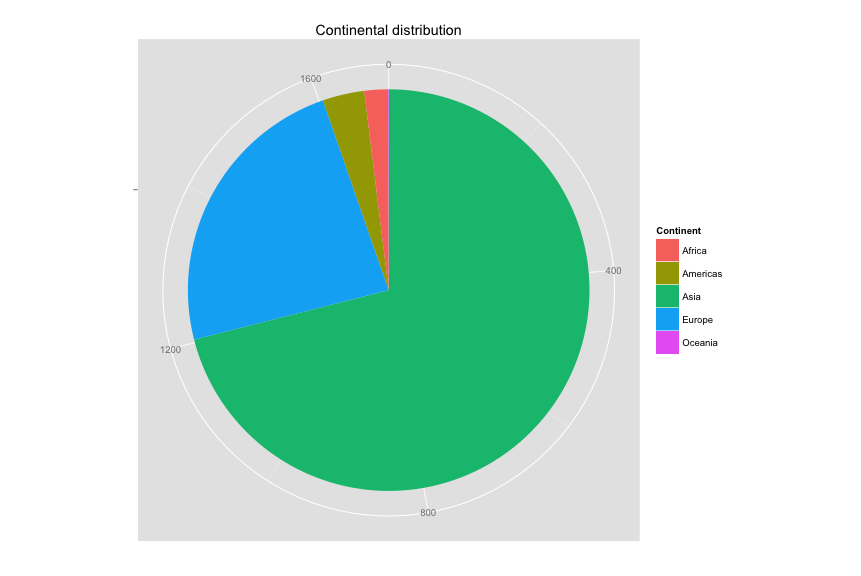
\includegraphics[width=\textwidth]{geo/ContinentalDist}
    \caption{Continents of participants on SportSense Crowdapp}
    \label{img:contDist}
\end{figure}

Figure \ref{img:contDist} shows the continental distribution of the workers and indicates that $71\%$ of the workers are from Asia.

\subsection{Time}

The following examines the time a user needs to finish a task.

\begin{figure}[H]
    \centering
    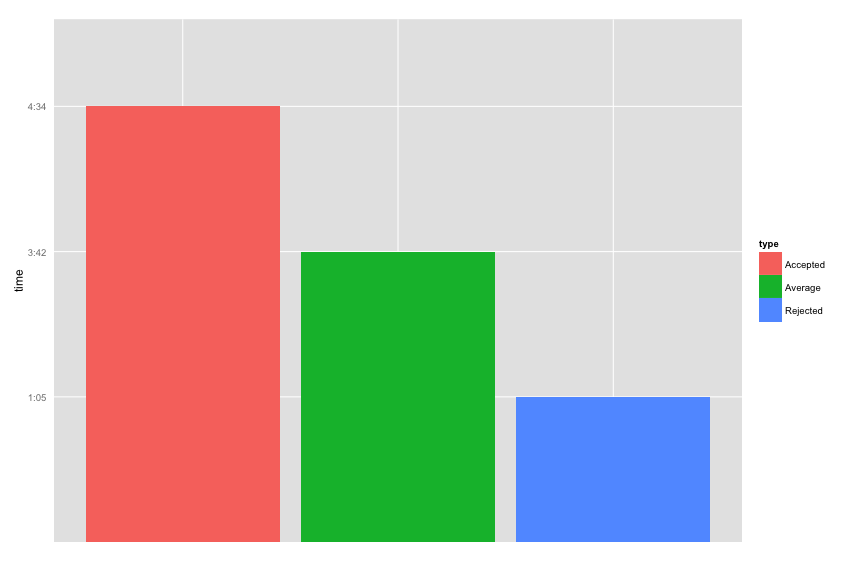
\includegraphics[width=\textwidth]{geo/TimeTask}
    \caption{Time users need to finish a task}
\end{figure}

The above figure shows that the average time for accepted tasks is substantially higher than the average time for not accepted tasks.
The average time for rejected tasks is 01:05, whereas the average time for accepted tasks is 4:34, which is about a quadruple of the time used by rejected tasks.





\newpage
\section{Conclusion}

Especially, the pretest \ref{sec:pretest} we have seen that many Microworkers users are not doing their task properly. Many users just finished the task without entering any events, if there have been some.
The pretest gave the possibility to eliminate those users from further tasks, because a user who did not enter any data will get a rating of $-1.5$, which is exactly the limit where users are not qualified to do more tasks.
\newline
By creating the tutorial video and playing it in the beginning, the tests also found that a smaller number of users had misunderstood the tasks.
\newline
There were also some difficult situations for the users, who were not clear about which event or how many events had to be entered, for example, the situation in a sequence of a player intercepting the ball and passing it at the same time to another player of his team. In this situation, three kinds of user inputs were made. The majority of users analyzing this sequence entered only an interception, the second most users entered only a pass, and there have also been some users entering a pass and an interception.
\newline
The calculation of the events in the two tests has shown that the DBSCAN algorithm works better than the UPGMA. However, the DBSCAN also produces mistakes and will not work if too many users enter inexact data, as it is only a statistical approach to calculate the clusters.
A big problem DBSCAN has in difficult situations is that it will join two different points to one if they are close enough to each other. As described in the example above the position, the time, and the team passing and intercepting is the same, only the event changed. This little difference cannot be detected as two separate events with the DBSCAN algorithm, because if the parameters are changed to something that it would accept, in this case there would be an overfitting for other points, and this will produce a large number of wrong points in other situations. Thus, false negative events are accepted, and the false positive are kept as small as possible to ensure that there should rather be non-existing events in the data instead of missing events.



